\chapter{Simple batch processing application}
\label{chapter_app}


This chapter describes a simple batch processing application that is used to demonstrate and validate the capabilities of the work presented in this thesis. The implementation of a simple application was chosen over an existing application for the ability to evaluate the work presented in this thesis in a controlled setting. The application described in this chapter is specifically designed to stress the CPU of a container. The quality of service described in SLOs of this application can thus be differentiated by regulating the allocated CPU.

\section{Design}
The design of the application is inspired by the architecture of the document processing application described in~\cite{Walraven2015b} and Pull Queues~\cite{pullqueue} available in Google App Engine.  The application consists of two major components: the Queue and Workers. The design is shown in Figure~\ref{fig:application1}.
\begin{figure}
    \centering
    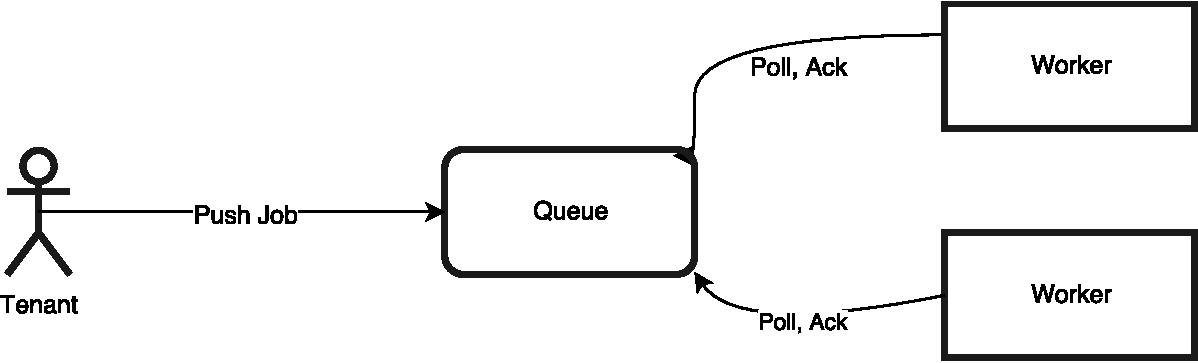
\includegraphics[width=0.6\textwidth]{chapter-artificial-application/queue1.pdf}
    \caption{Design simple batch processing application.}
    \label{fig:application1}
\end{figure}

\subsection{Queue}
The queue is used by tenants to submit jobs to the application via a publicly available interface. A job can consist of any amount of tasks of a specific type. Upon receiving a job, a unique reference for the job is created and the required tasks are added to the queue.\\
Tasks within the queue have a unique identifier and a reference to their corresponding job. The unique identifier is used by the workers to acknowledge a completed task. When a task was pulled by a worker but has not been acknowledged after a certain time interval, the task is re-queued. This simple mechanism allows to cope with the possible failure of workers. When all the tasks of a job are completed, the job is marked as completed. 

\subsection{Worker}
The worker component is responsible for the actual execution of a task. As by the pull design the worker will periodically poll the queue for work. Once a task is completed, the worker will poll the queue again. The result and identifier of the previous task are piggybacked by this poll. The type of work done by the worker is determined by the type of task.

\section{Implementation}
The components of the application are implemented as restful web services in the Java Spring Framework. 
\subsection{Queue}
As a web service the queue offers the following REST API to the tenants and the workers. 
\begin{itemize}
    \item \texttt{\textbackslash pushJob\textbackslash amount}: will push a job with a certain amount of tasks onto the queue as defined by the path parameter. 
    \item \texttt{\textbackslash pollTask\textbackslash acknowledge-task-uuid}: will poll the queue for a task. If a task is present within the queue, it will be returned as a JSON object. When a task identifier is specified as a path variable, the corresponding task will be successfully acknowledged. 
    \item \texttt{\textbackslash status}: returns a report about the current state of the queue. 
\end{itemize}

\noindent The tool described in Chapter~\ref{ch:k8-bench} requires the application to be testable by a load testing tool such as JMeter~\cite{jmeter}, Scalar~\cite{heyman2014scalability} or Locust~\cite{locust}.  The majority of load testing tools perform synchronous HTTP-request to evaluate the performance of a web application.  The synchronous nature of the HTTP-request implies that TCP connection is kept alive until a response is delivered to the tool. In the Spring framework, each HTTP-request is processed on a separate thread.  However the batch-oriented application described in this chapter works asynchronous (i.e, jobs placed in the queue are asynchronously processed by the workers) and the completion of jobs might take a considerable amount of time.  The connection and thus the thread must be kept alive during the entire execution of the job. This results in a build-up of active threads on the Queue component in the presence of multiple tenant requests. \\\\
To combine the synchronous nature of load testing tools with the asynchronous computation of the application, the concept of Java  \texttt{Future}~\cite{future} is utilized. When a job is submitted it is associated with a \texttt{Future}, blocking the thread responsible for the HTTP-request. A  \texttt{Future} allows the thread to be easily resumed (yielded) when the job has been marked completed by the queue.

\subsection{Worker}
The worker is implemented as a scheduled task from the Spring library. It will poll for a task after completing a task and each  fixed time interval (1 second). A poll is executed by a thread. A poll thread is stopped when no new tasks can be retrieved from the queue. However, additional threads can be spawned each time interval.   The currently implemented task execution for the worker stresses the CPU.\\\\
The implementation of the CPU stress test is inspired by the work of Matthews\textit{ et al.}~\cite{matthews2007quantifying} on quantifying the performance isolation of virtualization systems. The authors suggest to utilize a tight loop of integer arithmetic operations to individually stress the CPU.  The implemented stress test  shown in Listing~\ref{lst:cpustress} performs a loop of calculations in which the factorial of 30 is recursively calculated. The number of loops can be configured.

\begin{lstlisting}[caption=CPU stress test implementation., language=java, label={lst:cpustress}]
    public int run(){
        if(this.stressSize != 0){
            result = 0;
            for(int i =0 ; i < 100 * this.stressSize; i++){
                result = fac(30);
            }
        }
        return result;
    }

    private int fac(int n){
        if(n==1) {
            return 1;
        }
        else{
            int r =  fac(n-1);
            return r * n;
        }
    }
\end{lstlisting}

\section{Deployment in orchestration platform}
This section describes how the components are deployed within the container orchestration platform, Kubernetes. The deployment is shown in Figure~\ref{fig:queue2}.

\begin{figure}
    \centering
    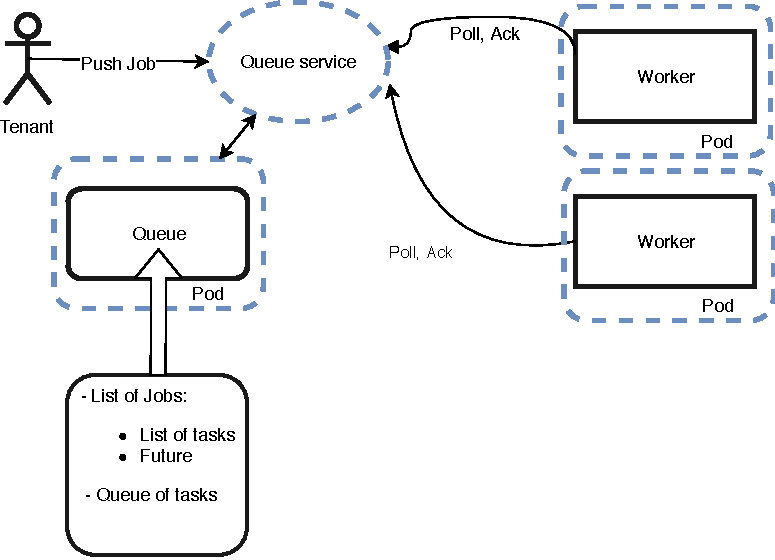
\includegraphics[width=0.6\textwidth]{chapter-artificial-application/deployment_artificial.pdf}
    \caption{Deployment of the simple batch processing application within a Kubernetes namespace.}
    \label{fig:queue2}
\end{figure}
\subsection{Queue}
The queue is deployed as a pod within a given namespace. The queue's REST API can be discovered/accessed via a Kubernetes service. 
\subsection{Worker}
The workers are deployed as pods part of a deployment within the same namespace as the queue. The workers use the Kubernetes DNS to discover the IP of the service coupled to the queue. The number of workers can be changed by the replica parameter of the deployment configuration.




